% 图 18.5 —— 由 `checks/emit_hand.py` 自动拼出（probe 精测 + prims2 图元分解）
%%
% ⚠ 这是**稿子不是成品**：跑 `checks/checkhand.py 18.5` 看指标 + 看叠合图。
%%
%% ⚠ 待核：
%   · 本图 probe 报出阴影族 1 个 —— **本脚本不生成阴影**（要照原书手写）；prims2 的 strokes 里可能含阴影线，核对时留意别画重
%   · 可疑字形 1 项（空心圈 ⊙ 常被认成字母 o）—— 见文件末
%%
\documentclass[12pt]{standalone}
\usepackage{fontspec}
\setsansfont{Arial}
\newfontfamily\mfallback{DejaVu Sans}
\usepackage{tikz}
\begin{document}
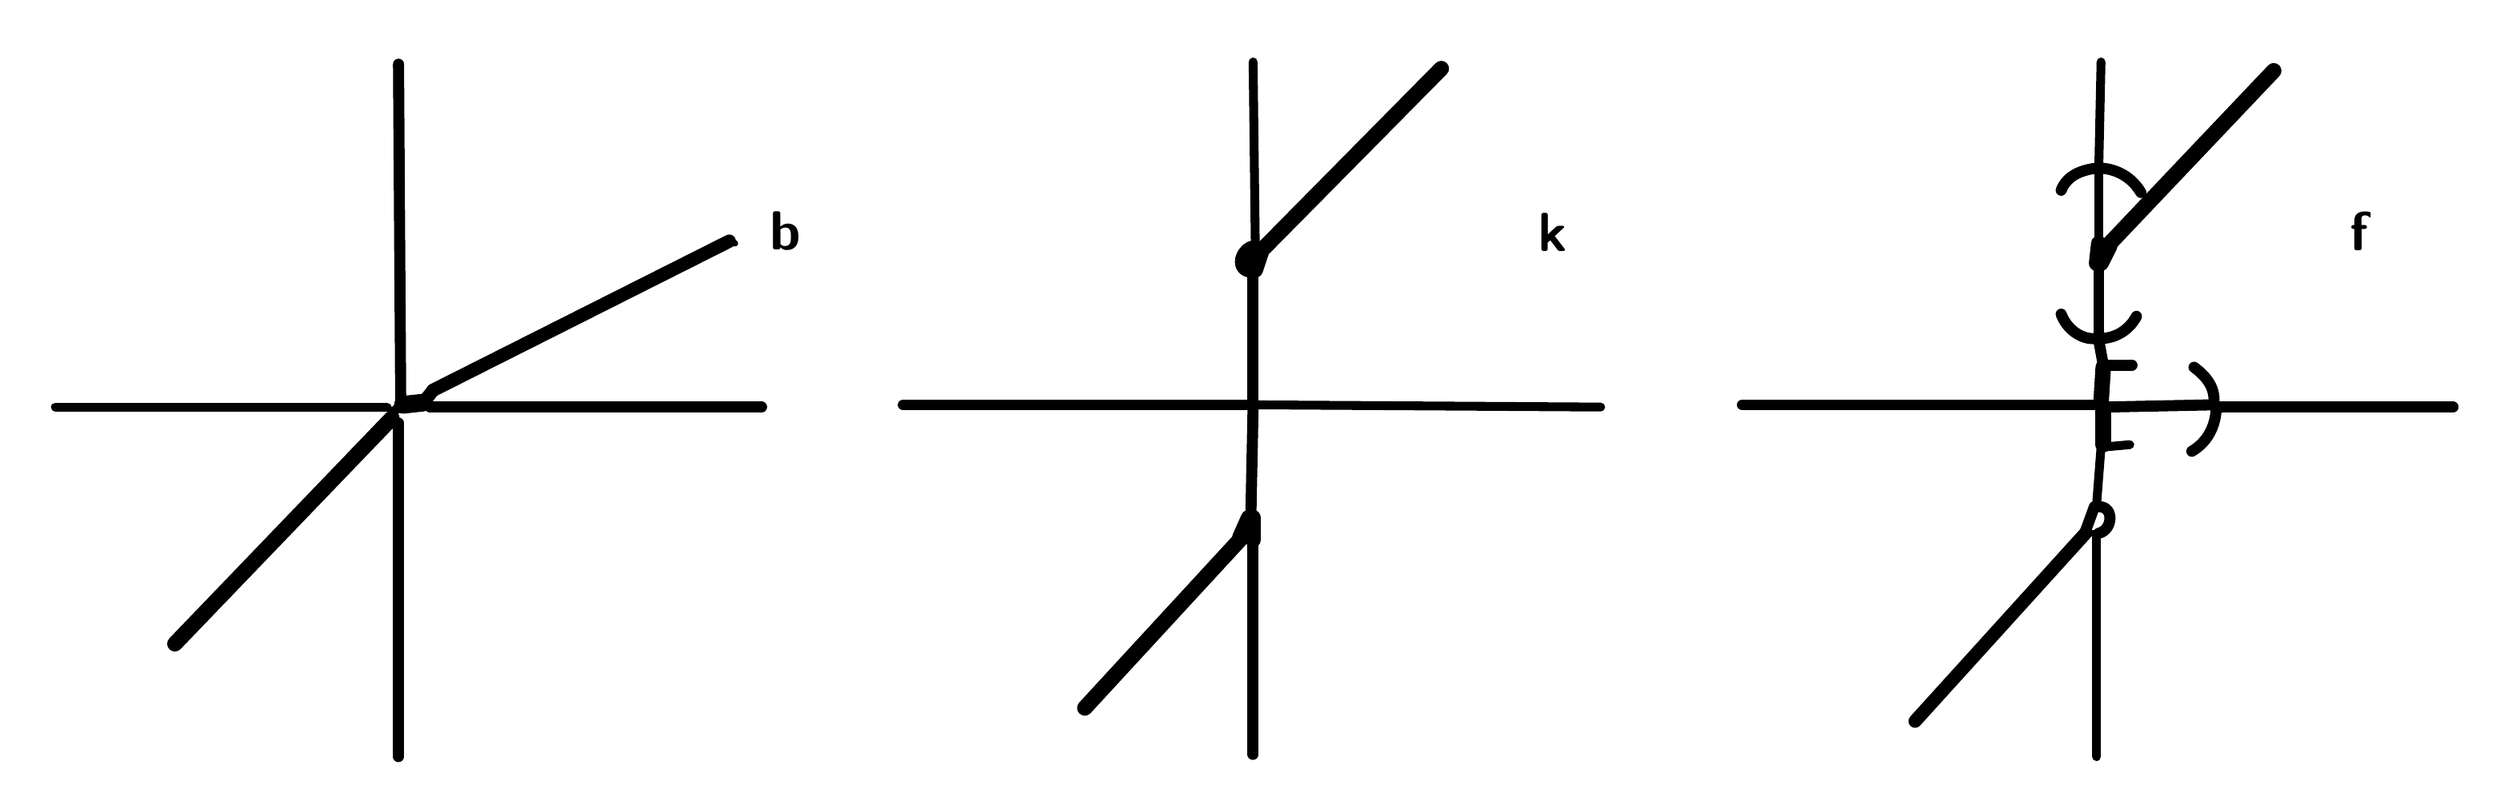
\begin{tikzpicture}[x=1pt, y=-1pt, line width=3.0pt, line cap=round, line join=round]

  %% ════ 直线段（prims2 的 strokes）════
  \draw[line width=3.0pt] (167.0,176.0) -- (164.8,174.0);
  \draw[line width=4.0pt] (164.8,174.0) -- (15.0,174.0);
  \draw[line width=6.0pt] (932.0,231.0) -- (855.0,316.0);
  \draw[line width=5.0pt] (940.0,155.0) -- (938.0,144.0);
  \draw[line width=5.0pt] (556.0,113.0) -- (556.0,172.0);
  \draw[line width=7.0pt] (556.0,234.0) -- (556.0,224.0);
  \draw[line width=4.0pt] (556.0,18.0) -- (557.0,101.0);
  \draw[line width=5.9pt] (182.0,171.0) -- (185.6,166.4);
  \draw[line width=6.0pt] (185.6,166.4) -- (319.4,99.0);
  \draw[line width=2.9pt] (319.4,99.0) -- (322.0,100.0);
  \draw[line width=5.0pt] (555.0,223.0) -- (556.0,174.0);
  \draw[line width=7.0pt] (554.0,224.0) -- (550.0,233.0);
  \draw[line width=5.0pt] (992.0,174.0) -- (1098.0,174.0);
  \draw[line width=3.0pt] (942.0,100.0) -- (939.0,100.0);
  \draw[line width=5.0pt] (556.0,235.0) -- (556.0,331.0);
  \draw[line width=5.0pt] (398.0,173.0) -- (555.0,173.0);
  \draw[line width=4.0pt] (937.0,332.0) -- (937.0,232.0);
  \draw[line width=8.0pt] (172.0,173.0) -- (181.0,172.0);
  \draw[line width=7.0pt] (940.0,156.0) -- (939.0,172.0);
  \draw[line width=7.0pt] (167.0,179.0) -- (69.0,281.0);
  \draw[line width=3.0pt] (936.0,231.0) -- (933.0,231.0);
  \draw[line width=4.0pt] (551.0,234.0) -- (555.0,234.0);
  \draw[line width=5.0pt] (953.0,155.0) -- (941.0,155.0);
  \draw[line width=3.0pt] (182.0,172.0) -- (184.2,174.0);
  \draw[line width=5.0pt] (184.2,174.0) -- (334.0,174.0);
  \draw[line width=5.0pt] (941.0,174.0) -- (989.0,173.0);
  \draw[line width=7.0pt] (940.0,175.0) -- (940.0,191.0);
  \draw[line width=7.0pt] (1017.0,22.0) -- (943.0,100.0);
  \draw[line width=7.0pt] (557.0,112.0) -- (560.0,103.0);
  \draw[line width=4.0pt] (938.0,99.0) -- (938.0,67.0);
  \draw[line width=5.0pt] (777.0,173.0) -- (938.0,173.0);
  \draw[line width=4.0pt] (938.0,65.0) -- (939.0,18.0);
  \draw[line width=4.0pt] (952.0,191.0) -- (941.0,192.0);
  \draw[line width=4.2pt] (171.0,173.0) -- (168.0,176.0);
  \draw[line width=7.0pt] (937.0,109.0) -- (938.0,100.0);
  \draw[line width=7.0pt] (550.0,234.0) -- (480.0,310.0);
  \draw[line width=5.0pt] (938.0,110.0) -- (938.0,142.0);
  \draw[line width=5.0pt] (936.0,219.0) -- (932.0,230.0);
  \draw[line width=5.0pt] (170.0,19.0) -- (171.0,172.0);
  \draw[line width=7.0pt] (939.0,109.0) -- (943.0,101.0);
  \draw[line width=7.0pt] (561.0,102.0) -- (641.0,21.0);
  \draw[line width=4.0pt] (557.0,173.0) -- (713.0,174.0);
  \draw[line width=4.0pt] (937.0,218.0) -- (939.0,192.0);
  \draw[line width=5.0pt] (170.0,332.0) -- (170.0,181.2);
  \draw[line width=3.0pt] (170.0,181.2) -- (168.0,179.0);

  %% ════ 曲线（prims2 的 curves —— 三段式，坐标同为 (y,x)）════
  \draw[line width=5.0pt] (981.0,156.0) .. controls (986.4,160.0) and (990.5,164.9) .. (990.0,172.0);
  \draw[line width=5.0pt] (937.0,66.0) .. controls (930.5,66.8) and (923.7,69.1) .. (921.0,76.0);
  \draw[line width=5.0pt] (921.0,132.0) .. controls (923.3,138.4) and (929.9,143.8) .. (937.0,143.0);
  \draw[line width=5.0pt] (938.0,231.0) .. controls (944.2,229.7) and (945.2,219.0) .. (938.0,219.0);
  \draw[line width=7.0pt] (557.0,102.0) .. controls (551.7,102.1) and (548.2,111.6) .. (555.0,112.0);
  \draw[line width=5.0pt] (939.0,143.0) .. controls (945.6,142.9) and (951.8,139.1) .. (955.0,133.0);
  \draw[line width=5.0pt] (939.0,66.0) .. controls (946.5,66.5) and (953.0,70.3) .. (957.0,77.0);
  \draw[line width=5.0pt] (980.0,194.0) .. controls (987.1,189.8) and (990.6,182.8) .. (991.0,175.0);

  %% ════ 标签（probe 直接给的 \node 行）════
  %% ⚠ 全部补了 fill=white：文字在最上层，否则与曲线交叉干扰
     \node[anchor=center,inner sep=0pt,fill=white,font=\fontsize{30.0}{37.5}\selectfont] at (344.8,94.2) {\textsf{\textbf{\textit{b}}}};   % box(335,82,17,22)
     \node[anchor=center,inner sep=0pt,fill=white,font=\fontsize{28.8}{36.0}\selectfont] at (691.2,94.9) {\textsf{\textbf{\textit{k}}}};   % box(683,83,16,21)
     \node[anchor=center,inner sep=0pt,fill=white,font=\fontsize{29.7}{37.2}\selectfont] at (1056.5,94.5) {\textsf{\textbf{\textit{f}}}};   % box(1050,83,12,22)

  % 钉死画布：否则超出的图元/控制点会把页面撑大，1:1 回比就失准
  \pgfresetboundingbox
  \path[use as bounding box] (0,0) rectangle (1109,342);
\end{tikzpicture}
\end{document}

% ⚠ 待核清单（probe 拿不准，人眼过一遍）：
%   · 未识别/跳过：⑤ 跳过/未识别的字形
